\documentclass{article}
\usepackage[utf8]{inputenc}
\usepackage{multicol}
\usepackage{graphicx}
\usepackage[a4paper, total={6in, 8in}]{geometry}
\graphicspath{ {./images/} }
\usepackage{listings}
\usepackage{color}
\usepackage{pgfplots}
\usepackage{amsmath}
\pgfplotsset{width=6.5cm,compat=1.9}

\definecolor{dkgreen}{rgb}{0,0.6,0}
\definecolor{gray}{rgb}{0.5,0.5,0.5}
\definecolor{mauve}{rgb}{0.58,0,0.82}

\lstset{frame=tb,
  language=Java,
  aboveskip=3mm,
  belowskip=3mm,
  showstringspaces=false,
  columns=flexible,
  basicstyle={\small\ttfamily}, 
  numbers=none,
  numberstyle=\tiny\color{gray},
  keywordstyle=\color{blue},
  commentstyle=\color{dkgreen},
  stringstyle=\color{mauve},
  breaklines=true,
  breakatwhitespace=true,
  tabsize=3
}

\usepackage{hyperref}
\hypersetup{
    colorlinks=true,
    linkcolor=black,
    filecolor=black,      
    urlcolor=black,
}

\urlstyle{same}

\title{\textbf{Find the longest common prefix from the given set of strings using Divide and Conquer Algorithm}}
\author{Kandagatla Meghana Santhoshi- IIB2019030,\\* Debasish Das - IIB2019031, \\* Surya Kant- IIB2019032 }
\date{Date: 13-03-2021}

\begin{document}
\maketitle
\begin{abstract}
In this paper we have discussed a Divide and Conquer
algorithm to find the longest common prefix from the given set of strings. We have also discussed the time and space complexity of the method.
\end{abstract}

\begin{multicols}{2}

\section{Problem}
Given a set of strings, you are tasked to find the longest common prefix from the set of strings and print prefix.

\section{Keywords}
Strings,Array of strings,Prefix,Longest Common Prefix(LCP),Divide and Conquer.

\section{Introduction}
From the word Divide and conquer,we can say conquering the required result by  dividing the larger elements into smaller ones.In this approach a problem is divided into smaller parts further into smaller problems divided and then solved till we reach base case.

This technique can be divided into the following three parts:

Divide- This involves dividing the problem into small sub problems.

Conquer- We will celebrate victory of the sub problem by calling further sub problems recursively until sub problem solved.

Combine- Given problems is solved by combining results from the recursively called sub problems.

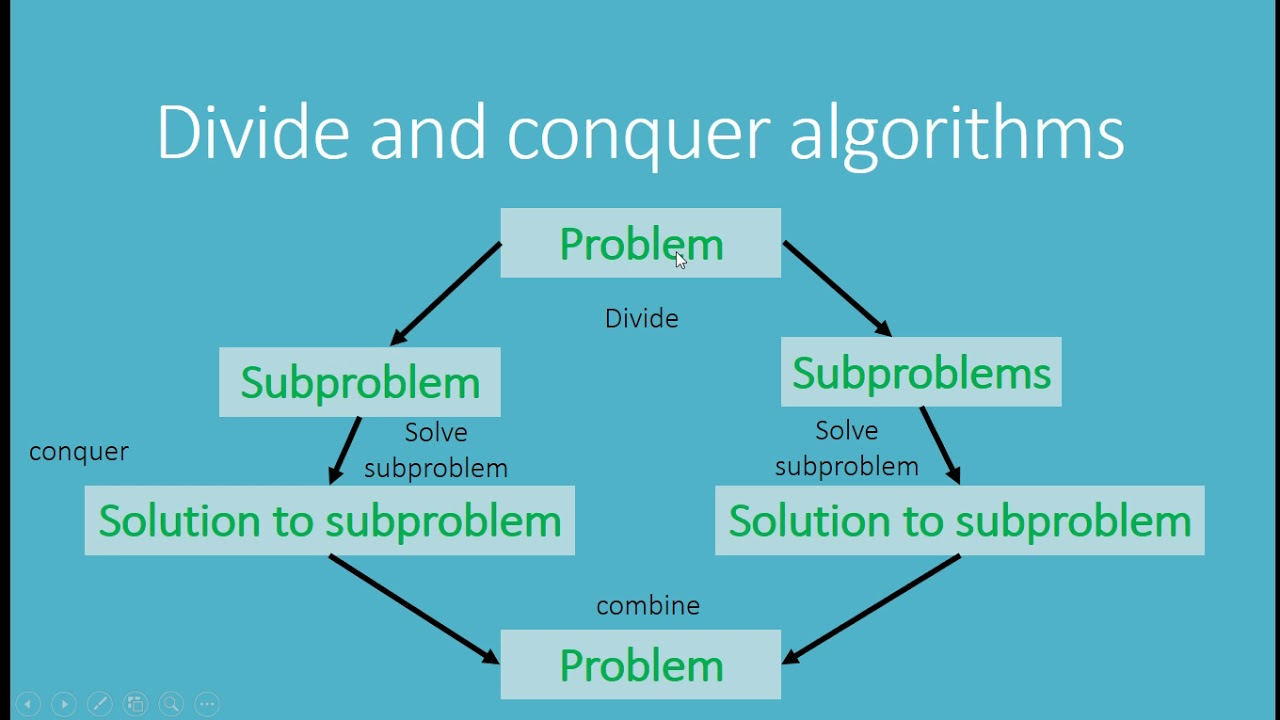
\includegraphics[scale=0.20]{Divide and Conquerjpg.jpg}
\begin{center}\textbf{Figure 1:}Divide and Conquer Methodology\end{center}

\section{Algorithm Analysis}
To find longest common prefix from the given set of strings:
 
\begin{enumerate}
\item We check if there is only one string,if yes clearly we return the whole string as LCP(Longest common prefix).Else We divide them into two sub problems.
\item Let us assume index to the middle element be mid,now we will find LCP of array of strings from start to mid and mid+1 to end.
\item Now we divide the strings of arrays till we reach the base case i.e,till start = end.
\item Then we try to find the common prefix from the returned strings of the sub problems.
\begin{itemize}
\item In this way, define a new subproblem with half the size of arrays and find Longest common prefix(LCP).
\end{itemize}
\end{enumerate}


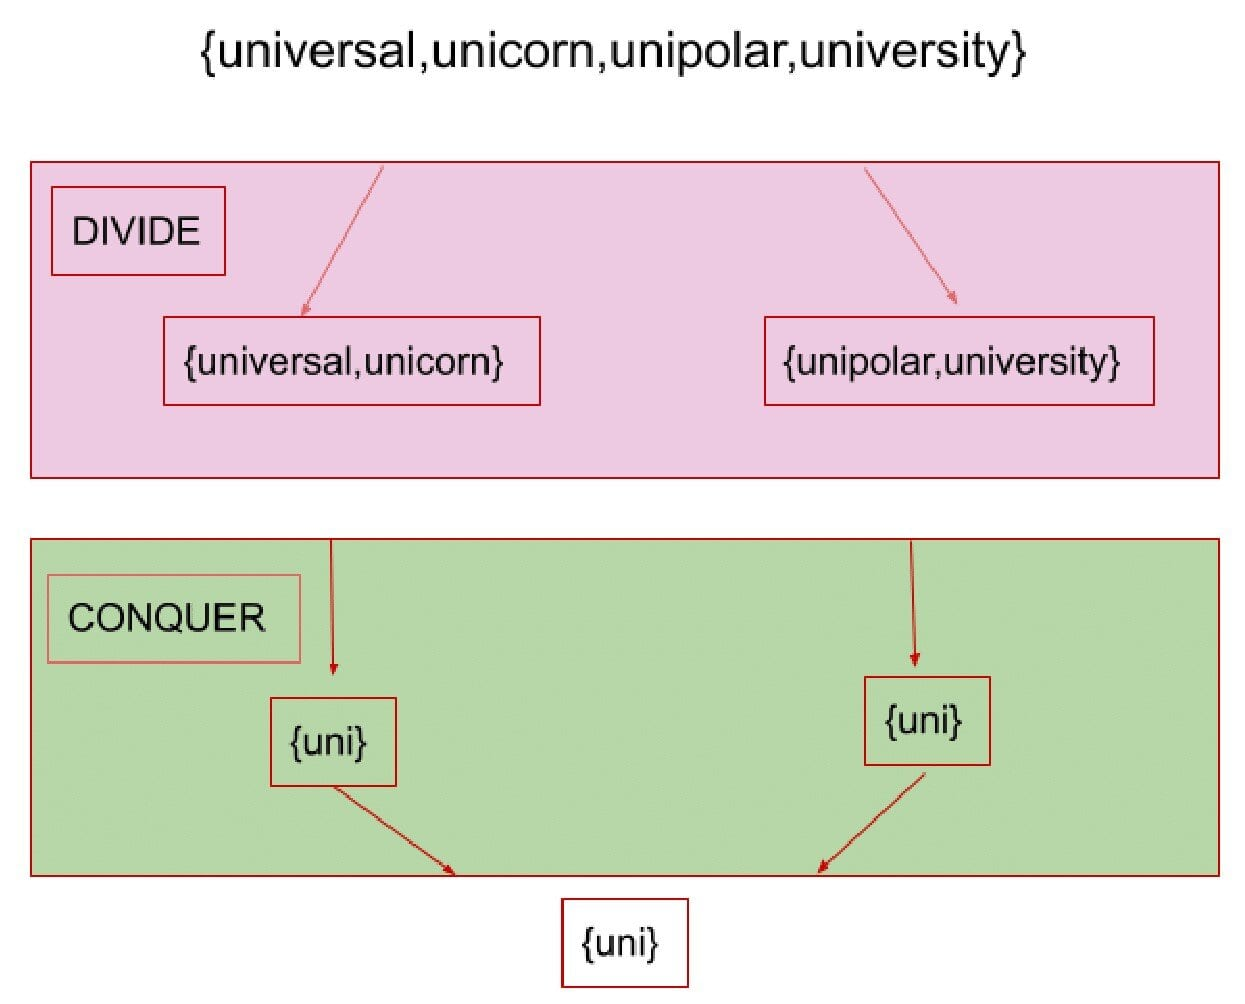
\includegraphics[scale=0.20]{example_as04.jpg}
\begin{center}\textbf{Figure 2:} Finding LCP using Divide and Conquer\end{center}

\section{Pseudo Code}
\lstset { %
    language=C++,
    backgroundcolor=\color{black!5},
    basicstyle=\footnotesize,
}

\begin{lstlisting}
arr[] has set of strings stored as an array,start and end are the variables used to point the start and end of arr[].string1,string2 strings to compare and find LCP.ans is the string used to store LCP of string 1 and string 2.

printArray Function:
    for i <- 0 to n
        print arr[i]

commonPrefix function:
    n1 <- size of string1 and n2 <- size of string2
    initialise i,j <- 0
    while(i<n1 && j<n2)
        if current character of string1 and string2 are equal
            include in common prefix => ans.push_back(string1[i])
            increment i and j => i++ and j++
        else 
            we break the while loop
    return ans
solveLCP function:
    if start = end 
        return arr[start]
    else if start > end
        return
    else 
        mid <- start+end/2
        string1 <- solveLCP(start,mid)
        string2 <- solveLCP(mid+1,end)
        
    return commonPrefix(string1,string2)
        
\end{lstlisting}

\subsection{Time Complexity Analysis}

We can observe that , we traversing every string in the given set of strings. Time complexity will be bigO(n*m) / O(n*m).Where n is Number of strings in the given set of strings and m is The longest string of all strings in the set.


\subsection{Space Complexity}

The space complexity of the Program is O(m*log(n)) Because of the space allocation for resultant strings in each subproblem.We can expect log(n) divisions.Each string returned by the subproblem can have maximum length of m.

\section{Experimental Analysis}
3D representation of time complexity are plotted :\newline
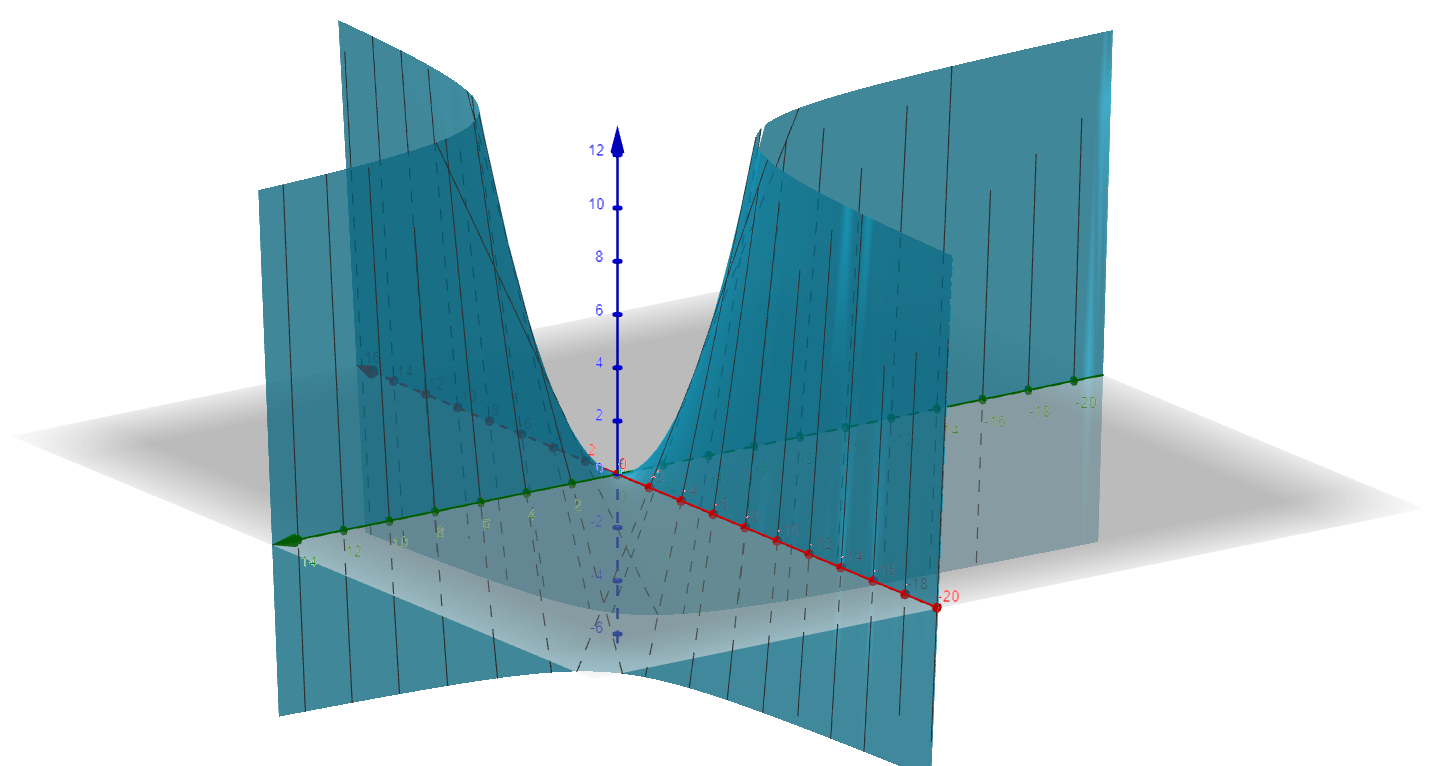
\includegraphics[scale=0.20]{time_plot.png}
\begin{center}\textbf{Figure 3:} Time Complexity O(n*m)\end{center}

3D representation of Space complexity are plotted :\newline
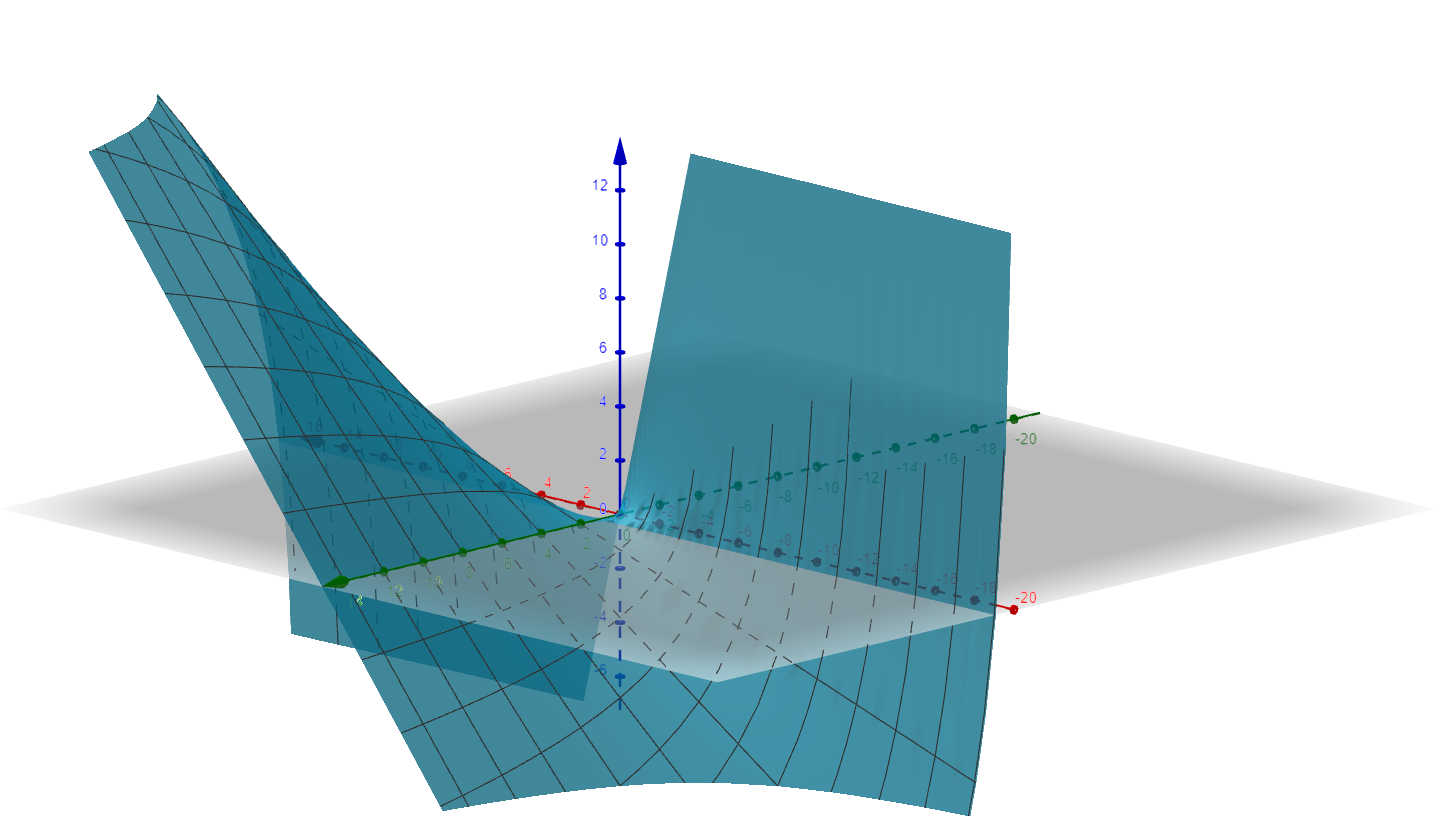
\includegraphics[scale=0.20]{space_plot.png}
\begin{center}\textbf{Figure 3:} Space Complexity O(m*log(n))\end{center}

\section{Conclusion}
Using Divide and Conquer algorithm , we have our time complexity to be O(n*m).\newline
This can be used in Constructing suffix tree , finding the number of occurrences in a pattern.

\section{Applications}
Divide and Conquer is a wide variety of algorithmic technique which believes on the strategy of division of the task and then combining them to form the required solution according to the requirement of the question.This methodology has many predefined algorithms which work on the basis of Divide and Conquer. Some of the applications of the Divide and Conquer Approach are:

\begin{enumerate}
\item \textbf{Merge Sort}
\item \textbf{Quick Sort}
\item \textbf{Binary Search} 
\item \textbf{Segment Trees} 
\item  \textbf{Strassen’s Algorithm} etc many more.
\end{enumerate}

\section{Acknowledgement}
We are very much grateful to our Course instructor Mr.Rahul kala and our mentor, Mr.Md Meraz, who have provided the great opportunity to do this wonderful work on the subject of Data Structure and Algorithm Analysis specifically on methodologies of Divide and Conquer.

\section{References}
\begin{enumerate}
1.Introduction to Algorithms by Thomas.H.cormen\newline
2.https://afteracademy.com/blog/longest-common-prefix\newline
3.https://afteracademy.com/blog/longest-common-prefix \newline
\end{enumerate}

\section{Appendix}
\subsection{Project link on Github:}
https://github.com/maggi2k19/DAA

\end{multicols}
\end{document}
